
\subsection{水治理指标间相关性变化}

分析综合治理指数(IWGI)及其三个子指标:稀缺情况(S)、使用目的(P)和分配方式(A)在三个不同时期,即集中供水时期(P1)、治理转变时期(P2)和适应增强时期(P3)的相关性,得到如下结果。

首先,我们关注 P1到P3 三个时段一起计算的相关性。结果表明 S 和 P 之间存在显著的负相关(相关系数为 $r = -0.75$,$p < 0.01$),说明此时期 S 和 P 之间具有较强的负向关系。
另一方面,A 和 IWGI 之间存在显著的正相关(相关系数为 $r = 0.75$,$p < 0.01$),表示 A 和 IWGI 之间具有较强的正向关系。然而,其他组合(如 S 和 A,S 和 IWGI,以及 P 和 A)的相关性在三个时段的总体上不具有统计显著性。

各时间段之间的相关性与上述整体趋势存在明显不一致(表\ref{ch4:tab:corr}),在集中供水时期(P1)内没有任何显著相关的指标组合。
而在治理转变时期(P2),S 和 P 之间存在显著的负相关(相关系数为 $r = -0.90$,$p < 0.01$),S 和 A 之间也存在显著的负相关(相关系数为 $r = -0.87$,$p < 0.01$),同时 P 和 A 之间存在显著的正相关(相关系数为 $r = 0.77$,$p < 0.01$)。
在适应增强时期(P3),S 和 P 之间、S 和 A 之间、以及 S 和 IWGI 之间的相关性均不具有统计显著性。然而,P 和 A 之间存在显著的负相关(相关系数为 $r = -0.86$,$p < 0.01$)。

\begin{figure}[!h]
    \centering
    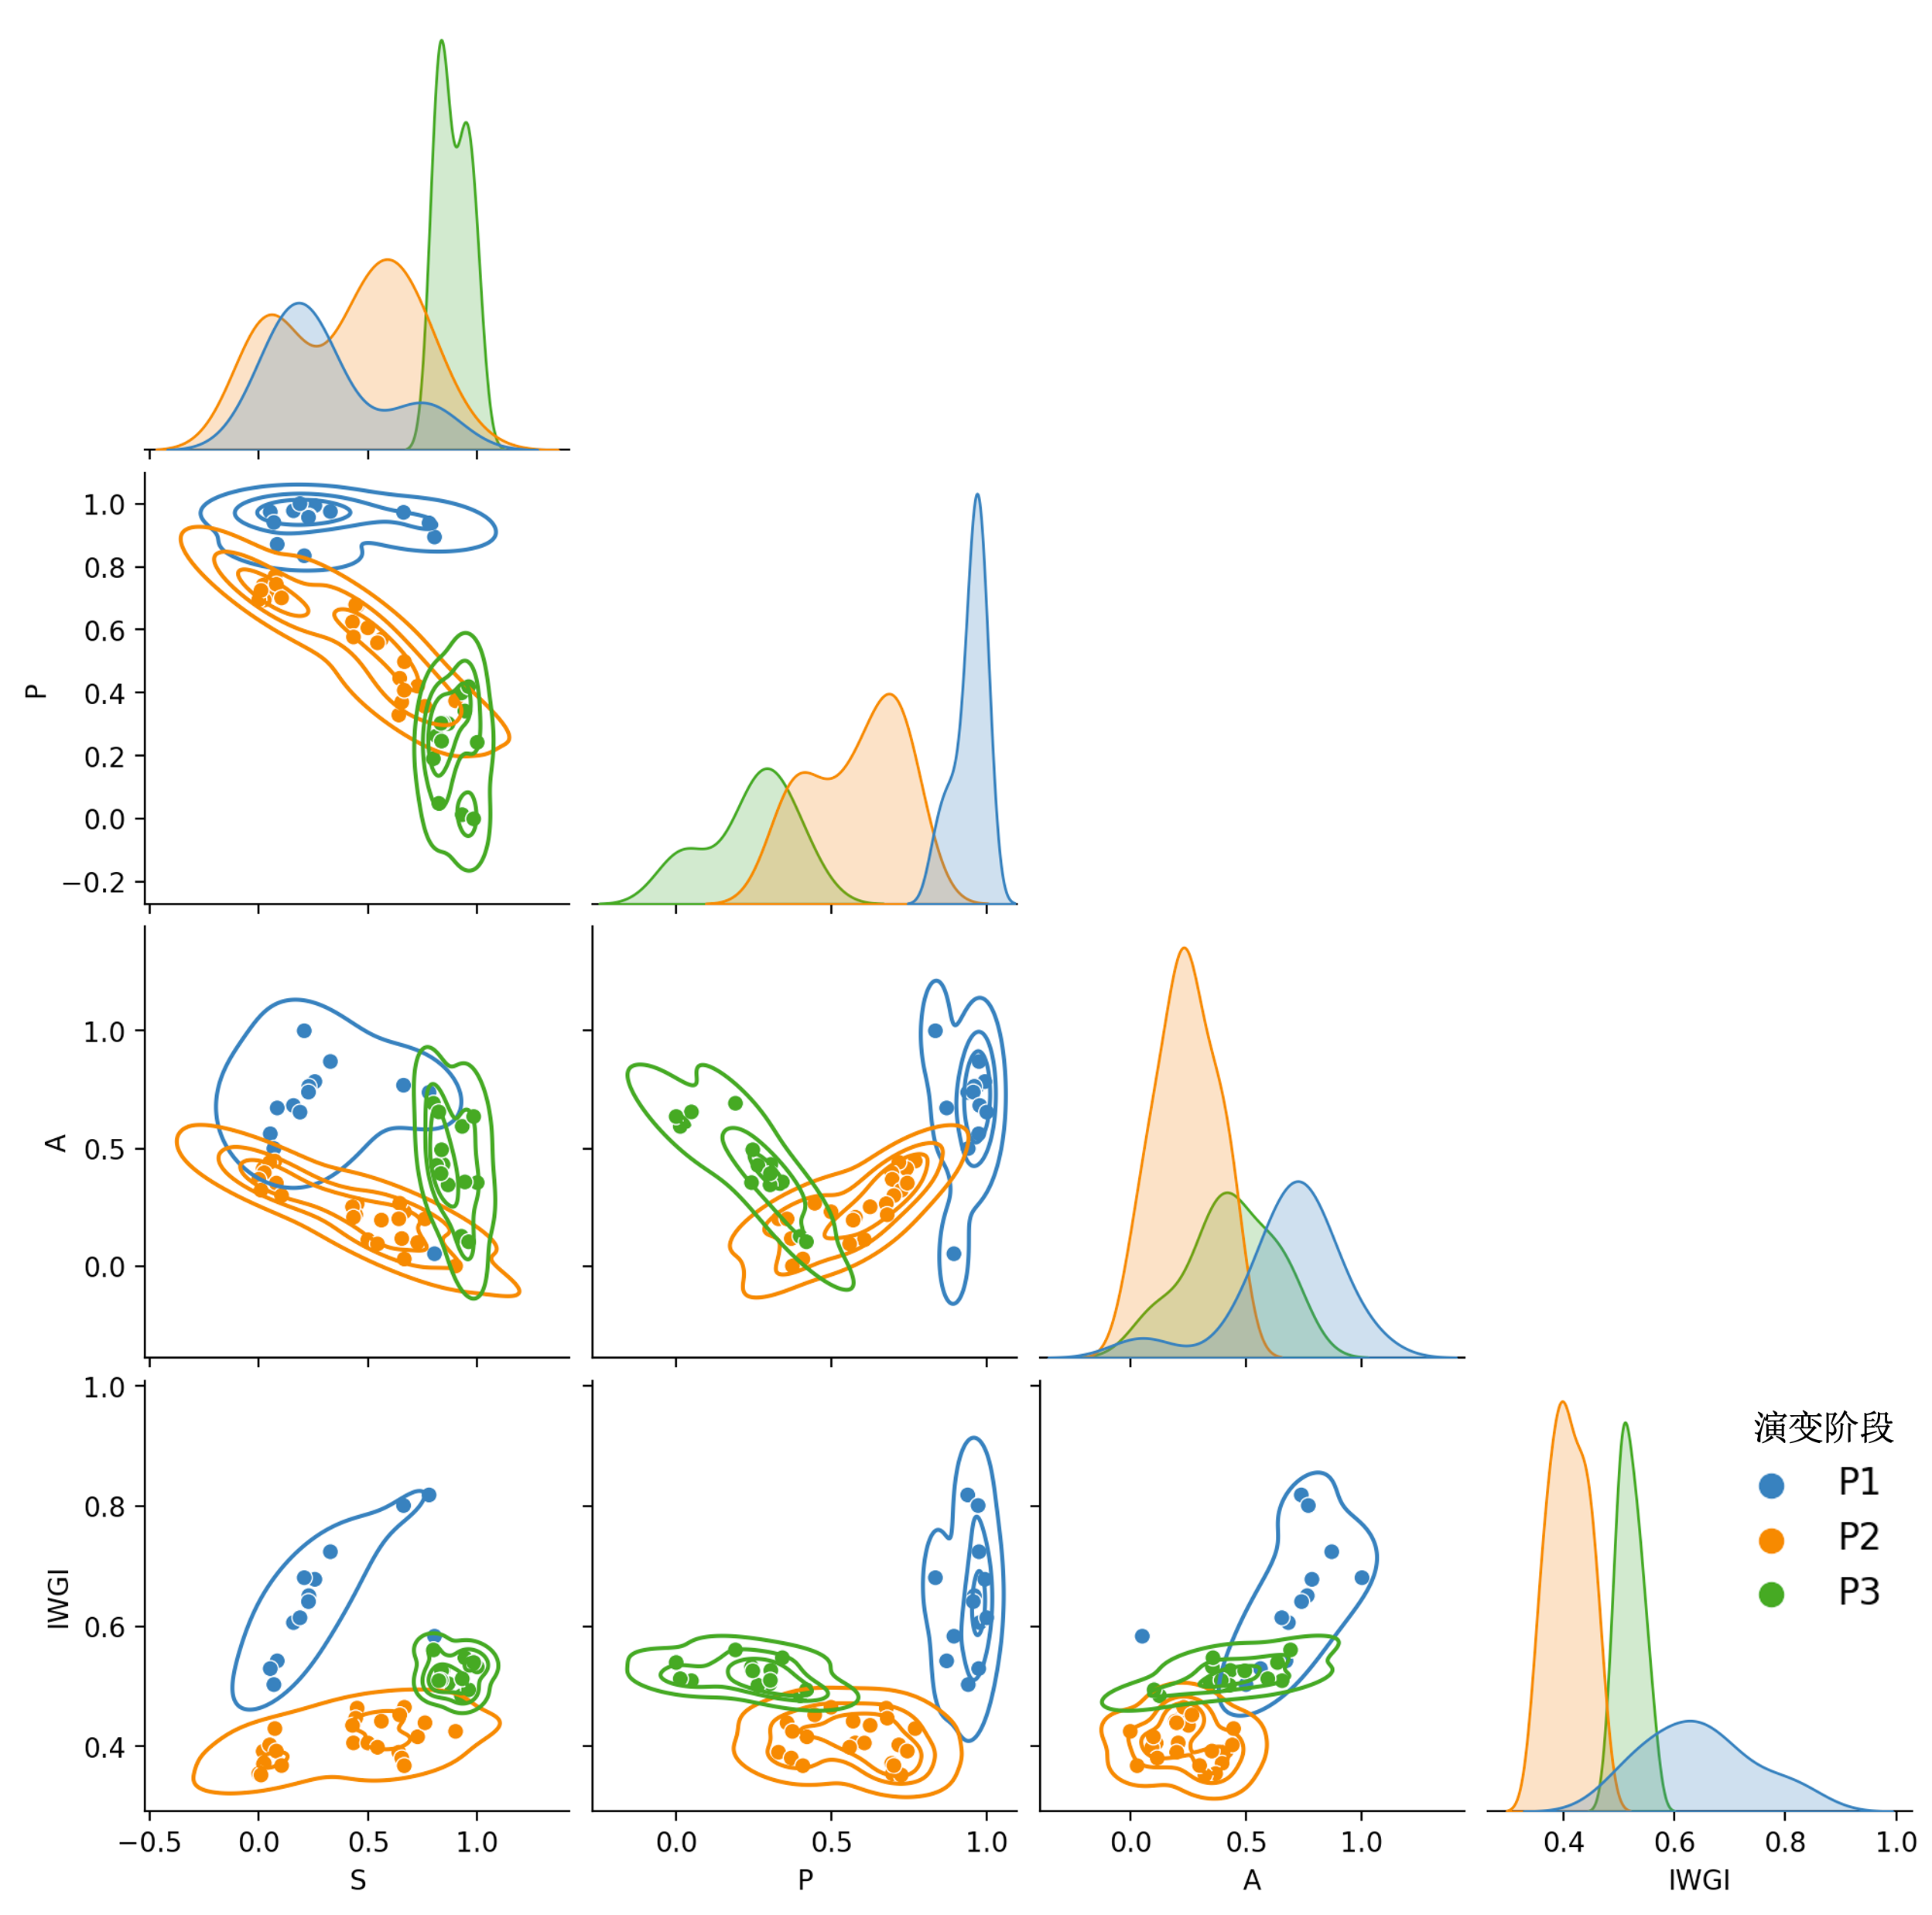
\includegraphics[width=\textwidth]{img/ch4/ch4_correlation.png}
    \caption{综合水治理指数IWGI及其各子指标间的相关性}\label{ch4:fig:corr}
\end{figure}

% Table generated by Excel2LaTeX from sheet '相关性情况'
\begin{table}[htbp]
    \centering
    \caption{综合治理指数(IWGI)及其三个子指标的相关性}
      \begin{tabularx}{\textwidth}{LLLLLLL}
      \toprule
      Period & \multicolumn{1}{l}{S vs P} & \multicolumn{1}{l}{S vs A} & P vs A & \multicolumn{1}{l}{P vs IWGI} & \multicolumn{1}{l}{A vs IWGI} & \multicolumn{1}{l}{S vs IWGI} \\
      \midrule
      P1 - P3 & \multicolumn{1}{l}{-0.75 *} & -0.29 & 0.36 & 0.37  & \multicolumn{1}{l}{0.75 *} & 0.14 \\
      P1    & -0.08 & -0.31 & 0.06 & 0.14  & 0.51  & 0.65 \\
      P2    & \multicolumn{1}{l}{-0.90 *} & \multicolumn{1}{l}{-0.87 *} & 0.77 * & -0.18 & -0.13 & 0.5 \\
      P3    & 0     & -0.38 & -0.86 * & -0.33 & 0.61  & 0 \\
      \bottomrule
      \end{tabularx}%
    \label{ch4:tab:corr}%
  \end{table}%


% \begin{figure}[!h]
%     \centering
%     \includegraphics[width=\textwidth]{img/ch4/ch4_P1_corr.png}
%     \caption{集中供水时期综合水治理指数IWGI及其各子指标间的相关性}\label{ch4:fig:corr}
% \end{figure}

% \begin{figure}[!h]
%     \centering
%     \includegraphics[width=\textwidth]{img/ch4/ch4_P2_corr.png}
%     \caption{治理转变时期综合水治理指数IWGI及其各子指标间的相关性}\label{ch4:fig:corr}
% \end{figure}

% \begin{figure}[!h]
%     \centering
%     \includegraphics[width=\textwidth]{img/ch4/ch4_P3_corr.png}
%     \caption{适应增强时期综合水治理指数IWGI及其各子指标间的相关性}\label{ch4:fig:corr}
% \end{figure}

\subsection{水治理变化的驱动力分析}\label{ch4:sec:mechanism}

\begin{figure}[th!]
	\centering
	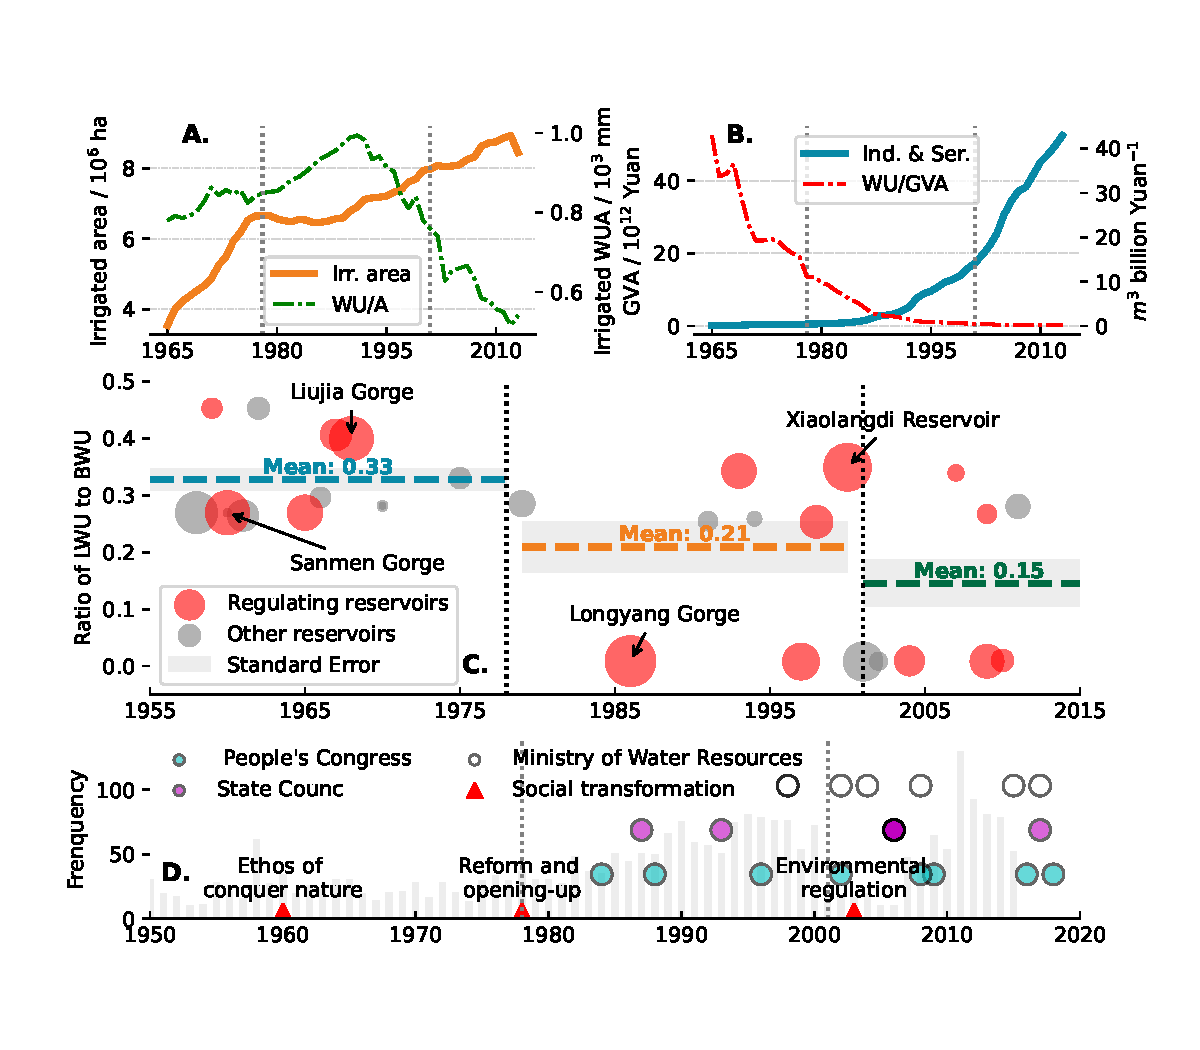
\includegraphics[width=\textwidth]{img/ch4/causes.pdf}
	\caption[黄河流域水治理阶段变化的驱动因素]{
		黄河流域水治理阶段变化的驱动因素。
		\textbf{A.}总灌溉面积($A$, 橙色线)和用水强度($WU/A$,用水量除以灌溉面积,绿点线)的变化。
        \textbf{B.}工业和服务业的总增加值(蓝线,$GVA$)变化及其用水强度($WU/GVA$,$WU$除以$GVA$,红点线)。
        \textbf{C.}每个水库的完工时间及其所在区域的用水量(Local Water Use, $LWU$)占水库完工时流域总用水量(Basinal Water Use, $BWU$)的百分比。红圈为负责黄河流域综合调度的水库。每个圆圈的大小表示其储水能力的大小。
        \textbf{D.}社会转型(红色三角形)和国家层面的治理政策(圆圈,不同颜色表示由不同的国家机构签署,越靠上代表国家机构的等级越高,详见表\ref{ch4:tab:policies})。浅灰色条形图以流域尺度(黄河大事件)计算与黄河流域有关的官方治理文献记录。}\label{ch4:fig:mechanism}
\end{figure}


\begin{figure}[tb]
    \centering
    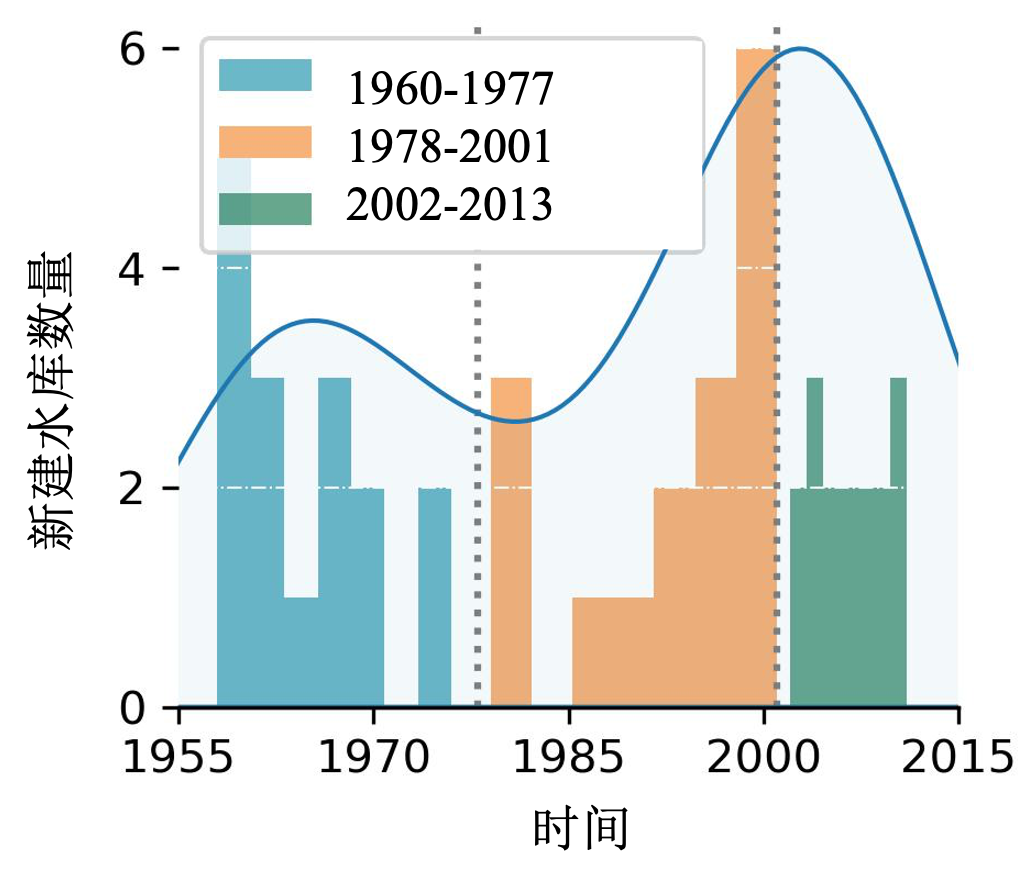
\includegraphics[width=0.6\linewidth]{img/ch4/ch4_reservoirs.png}
    \caption{黄河流域新增水库数量的时间分布}\label{ch4:fig:reservoirs}
\end{figure}


本节进一步探讨了致使IWGI变化的原因,灌溉区扩张和工业和服务业的经济增长是推动“集中供水时期”和“治理转变时期”两个阶段变化的关键。
黄河流域的用水需求在“集中供水时期”迅速增加,尤其是灌溉农业面积以$0.25*10^6~ha/yr$的速度迅速扩张(图\ref{ch4:fig:mechanism}~A),同时各地区大力建设水库增加水资源供应(图~\ref{ch4:fig:reservoirs})。
进入“治理转变时期”后,尽管灌溉区扩张停滞,但工业和服务业的发展开始增长,共同推动流域用水需求的进一步增加(图\ref{ch4:fig:mechanism}~A和B)。
接下来从“治理转变时期”到“适应增强时期”的演变过程中,径流量的不断下降是研究时段内水资源压力上升的原因之一(图\ref{ch4:fig:natural}),水分利用效率变化也起到非常明显的作用(图\ref{ch4:fig:mechanism}A和B)。
在“适应增强时期”,工业和城市服务承担了更重要的经济角色(由总增加值GVA表示,图\ref{ch4:fig:mechanism}~B),灌溉面积也恢复了缓慢扩张(图\ref{ch4:fig:mechanism}~A)。
但因用水效率的普遍提高,单位灌溉面积或单位产量的用水量都显著下降(图~\ref{ch4:fig:mechanism}~A和图~\ref{ch4:fig:mechanism}~B),因此部门和地区之间的用水差异在不断缩小,但流域水资源压力总体、持续维持在较高水平,如何公平合理分配宝贵水资源的挑战越来越大(图~\ref{ch4:fig:IWGI}~A)。

\begin{figure}[!h]
	\centering
	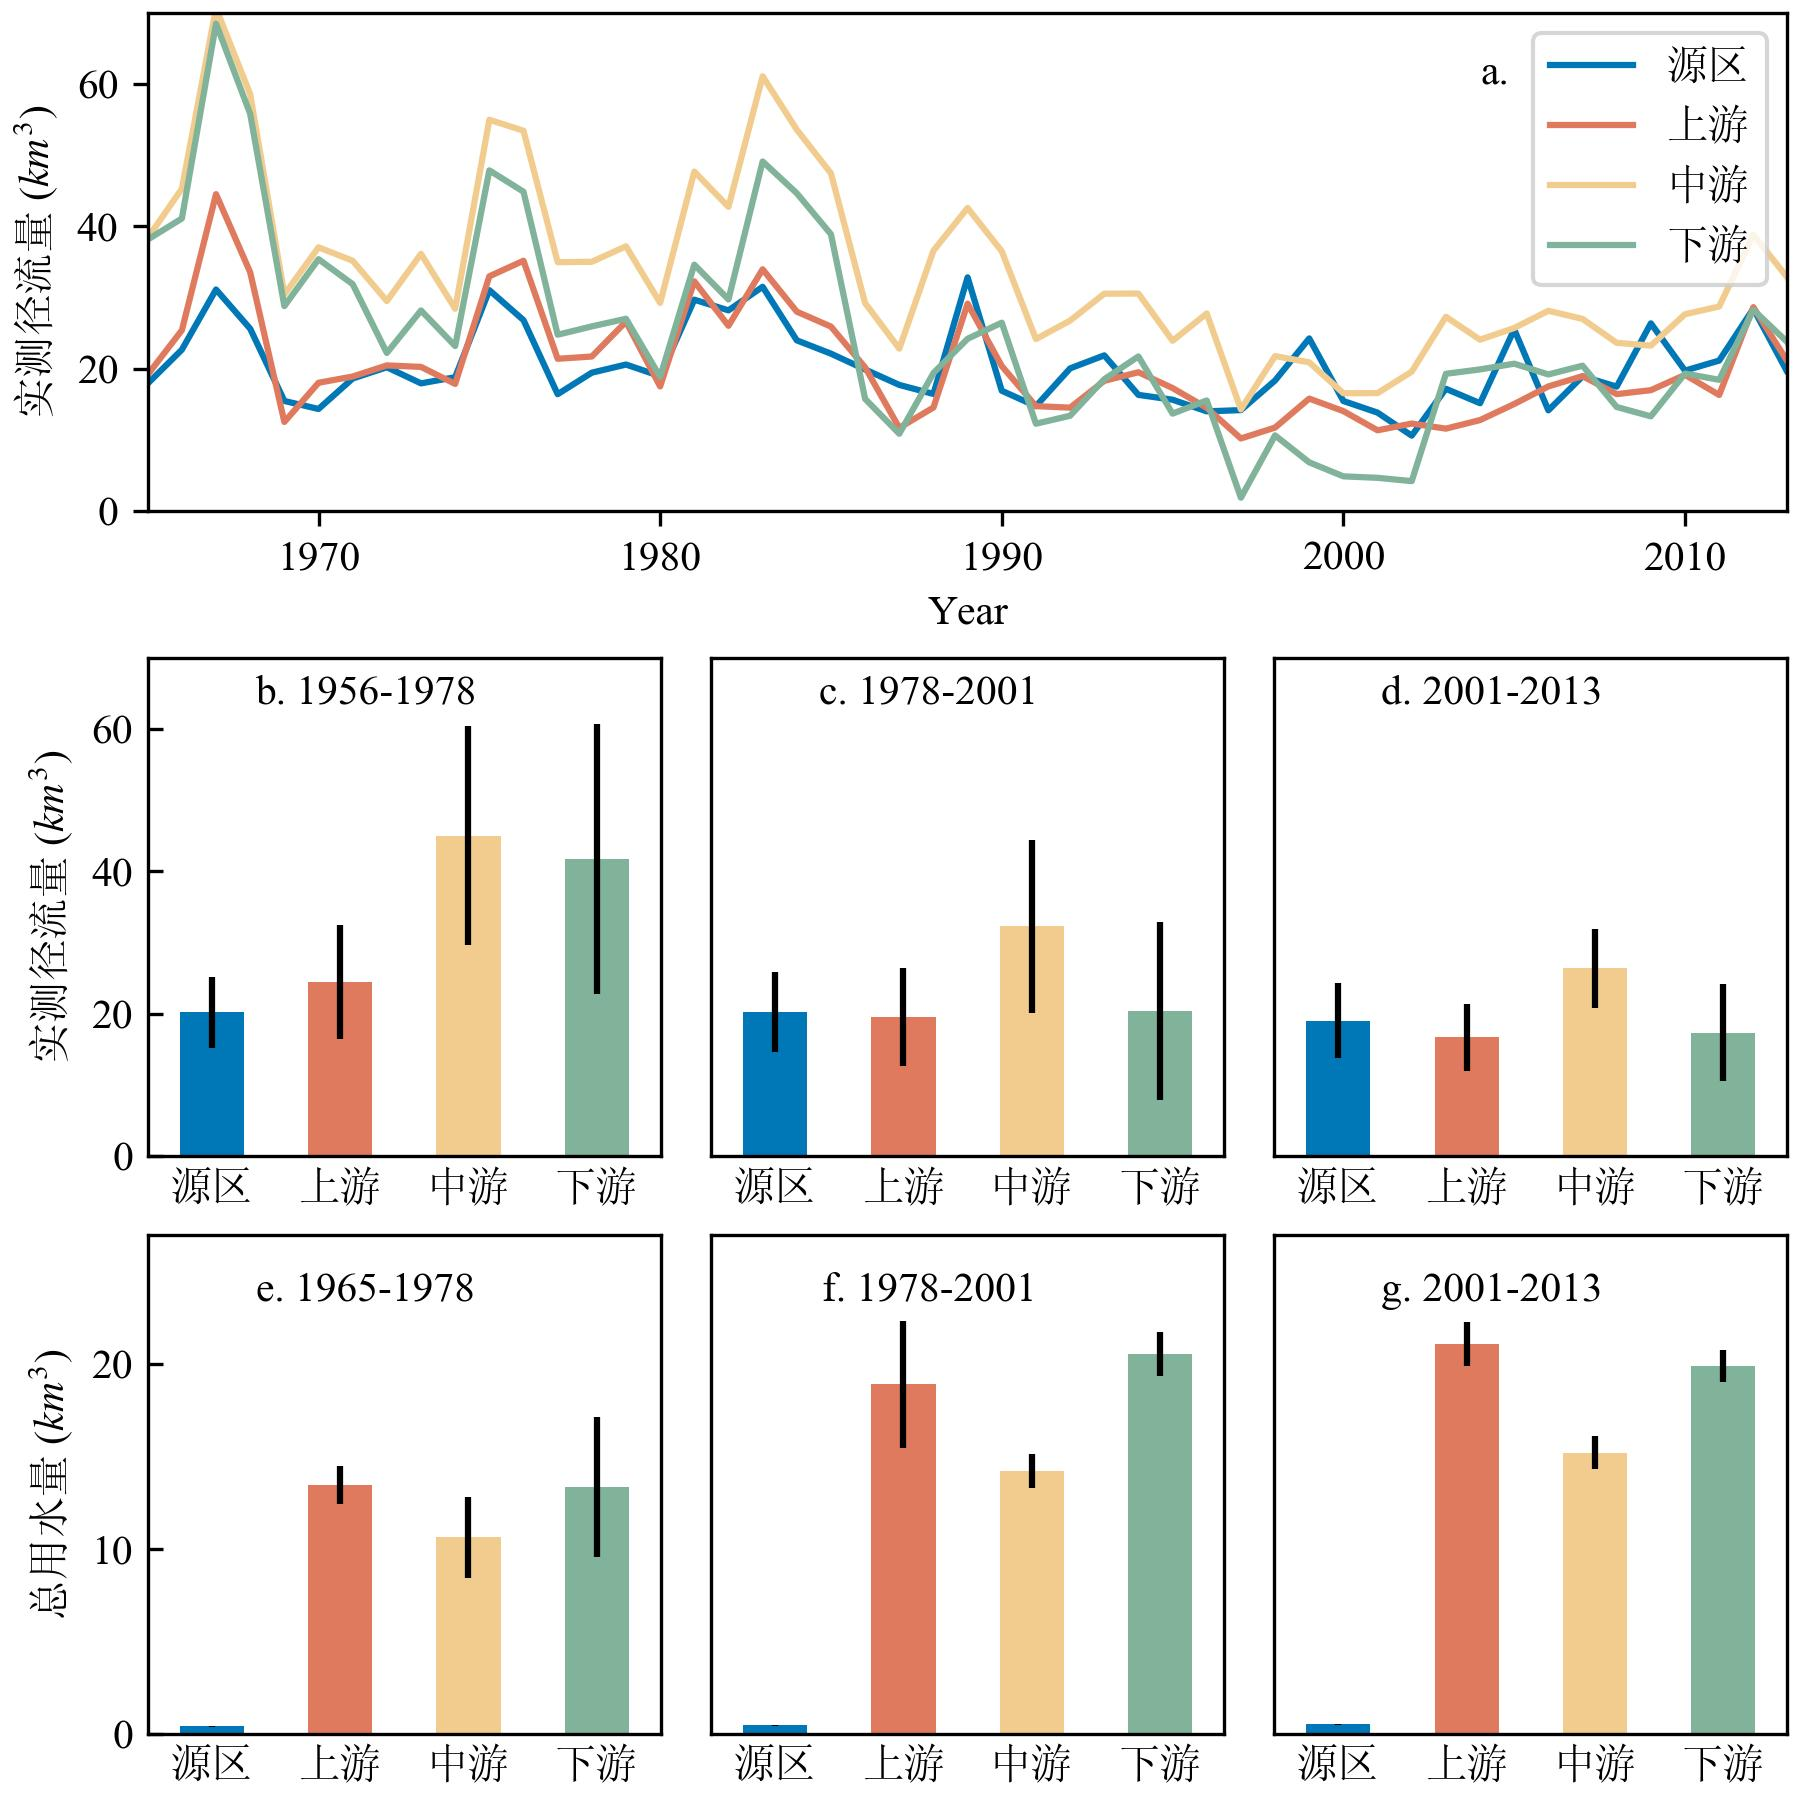
\includegraphics[width=\textwidth]{img/ch4/ch4_natural_water.jpg}
	\caption[黄河流域各区域天然径流量及水资源量分阶段变化]{
        黄河流域各区域天然径流量及水资源量分阶段变化。
        \textbf{a.} 实测径流量多年变化趋势。
        \textbf{b.} 集中供应时期不同地区的实测径流量。
        \textbf{c.} 治理转型时期不同地区的实测径流量。
        \textbf{d.} 适应增强时期不同地区的实测径流量。
        \textbf{e.} 集中供应时期不同地区的用水量。
        \textbf{f.} 治理转型时期不同地区的用水量。
        \textbf{g.} 适应增强时期不同地区的用水量。
    }\label{ch4:fig:natural}
\end{figure}

最后,环境背景、社会文化、水治理政策等因素对三个时期的指标变化都产生了影响。
每个水库的区域用水量和流域用水量之比可一定程度上反映修建水库对流域水治理的影响,较高的比值代表了该水库的潜在作用更倾向于为该流域供水;主要负责流域调度的枢纽水库则标记为红色(图~\ref{ch4:fig:mechanism}~C)。
可以看到,在阶段一的“集中供水时期”,受“人定胜天”的社会环境引领,大部分水库都建在需水量较大的地区,因此区域用水量和流域用水量之比值明显较高($p<0.01$,见图~\ref{ch4:fig:mechanism}~C)。
进入“治理转变时期”之后,新建水库的数量明显减少且多为枢纽水库。
此时期流域尺度的法律法规和流域内的治理记录也开始迅速增加,可见此时期层出不穷的流域政策已深刻影响了流域水治理,标志着流域水治理正在进行一场从工程措施向非工程措施的“治理转变”(图~\ref{ch4:fig:mechanism}~D, $p<0.01$和图\ref{ch4:fig:reservoirs})。
最后,在“适应增强时期”,持续高位的水压力已成为制约区域发展的瓶颈,亟需通过节水转型和跨区域协调、调水来满足经济发展的用水需求。
在“大规模进行环境治理和节水转型”的国家战略指导下,有关部门此时期也提出了更多的、级别更高的水治理决策(图~\ref{ch4:fig:mechanism}~D)。
综上所述,从“集中供水时期”到“治理转变时期”的转变与当时水资源供需的增加相一致;而“治理转变时期”到“适应增强时期”的演变过程则是在水资源压力趋于稳定的同时,由社会监管政策和节水转型带来的效率提高所驱动的。
